
\subsection{First Come First Served}
\markright{\thesubsection\quad First Come First Served} % Manually update \rightmark

\subsubsection{Turnaround time}

From \cref{fig:fcfsTurnEcdf} and \cref{fig:fcfsTurnDensity} we can see that a larger $\rho$ skews the distribution of turnaround time to the right. The effects of $\rho$ are more pronounced with fewer CPUs, and a higher \texttt{pCpuBound}. This can be explained by the fact that, with a higher \texttt{pCpuBound} a process spends most of its time in the CPU, increasing the probability of forming a queue of ready processes.  

\begin{figure}[H]
    \captionsetup{type=figure}
    \centering
    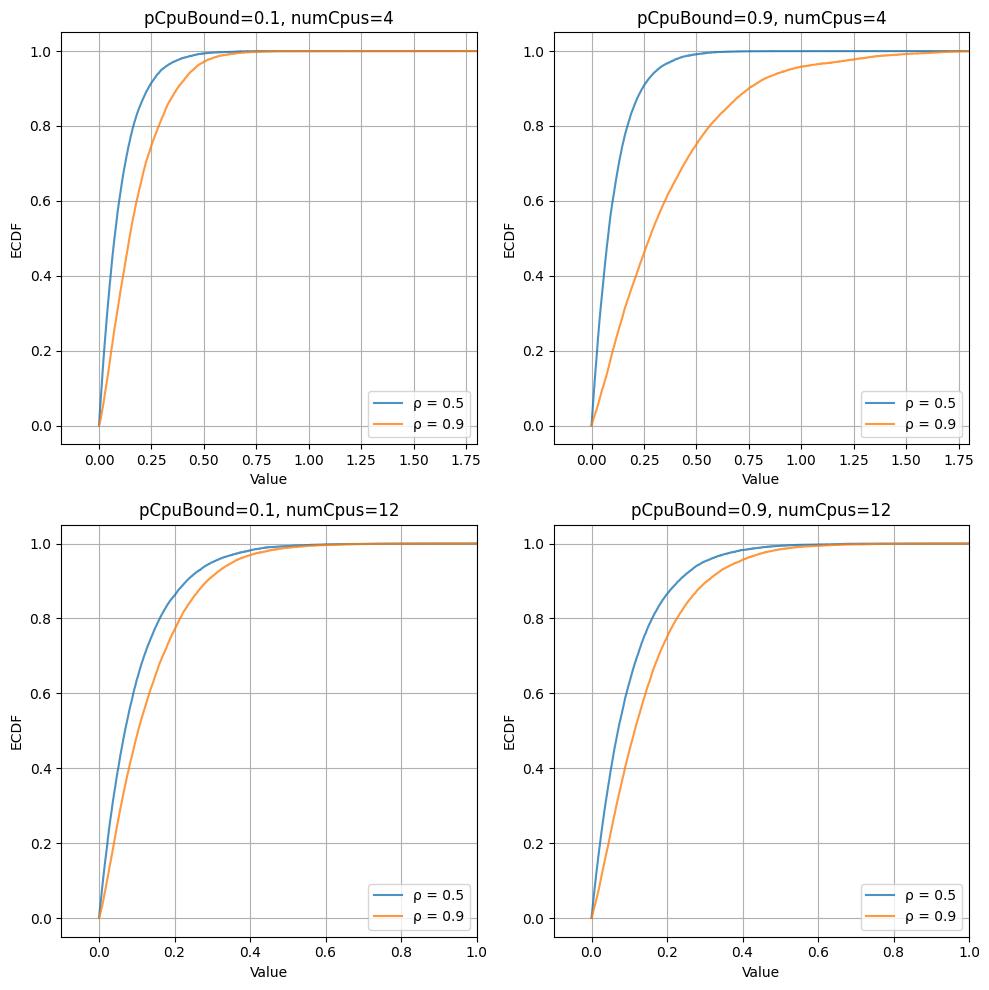
\includegraphics[width=0.9\textwidth]{./images/04/fcfs/turn/ecdf.png}
    \caption{Empirical CDF of the turnaround time of the systems.}
    \label{fig:fcfsTurnEcdf}
\end{figure}

\begin{figure}[H]
    \captionsetup{type=figure}
    \centering
    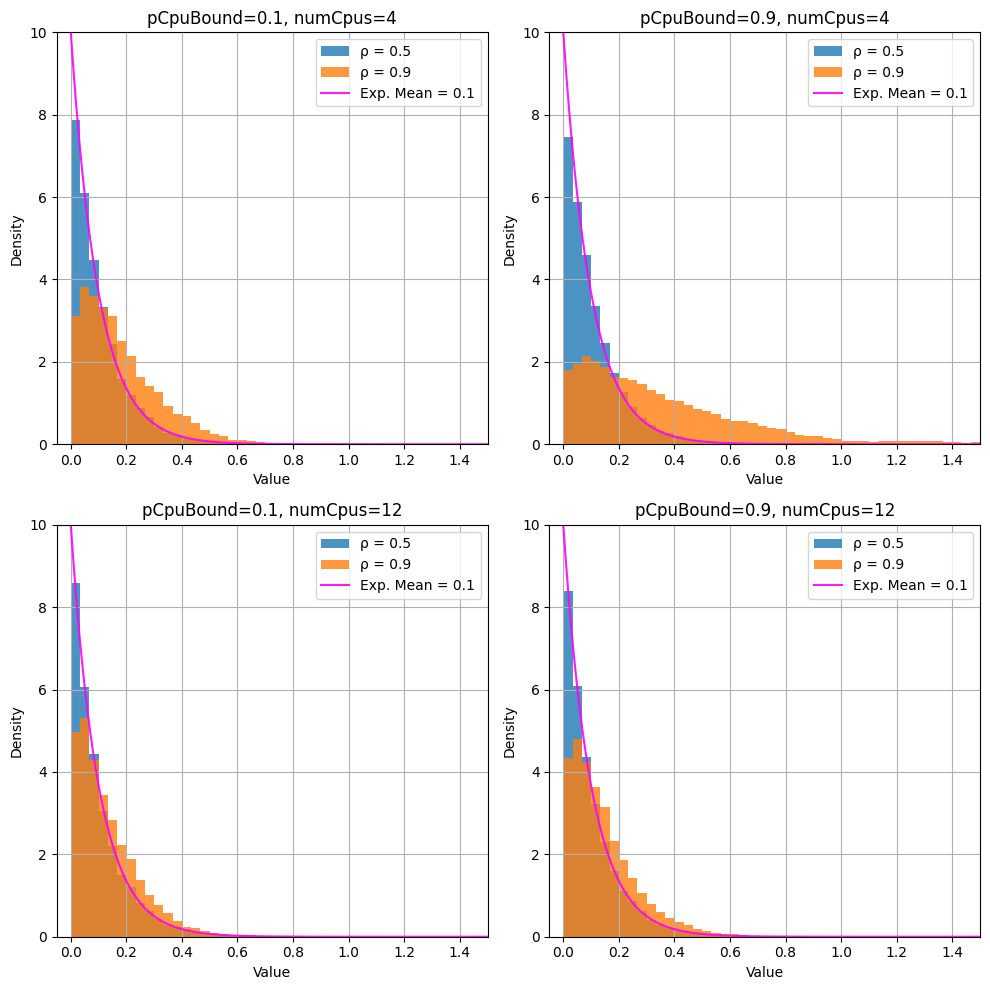
\includegraphics[width=0.9\textwidth]{./images/04/fcfs/turn/density.png}
    \caption{Density plot of the turnaround time of the systems.}
    \label{fig:fcfsTurnDensity}
\end{figure}

From the lorenz curve in \cref{fig:fcfsTurnLorenz} we can see that the distribution that the turnaround time assumes with bigger $\rho$ is more fair than the one with smaller $\rho$. In \cref{fig:fcfsTurnAutocorrelation} we see that larger $\rho$ values make the distribution more correlated, while more CPUs and a lower \texttt{pCpuBound} make the distribution less correlated.

\begin{figure}[H]
    \captionsetup{type=figure}
    \centering
    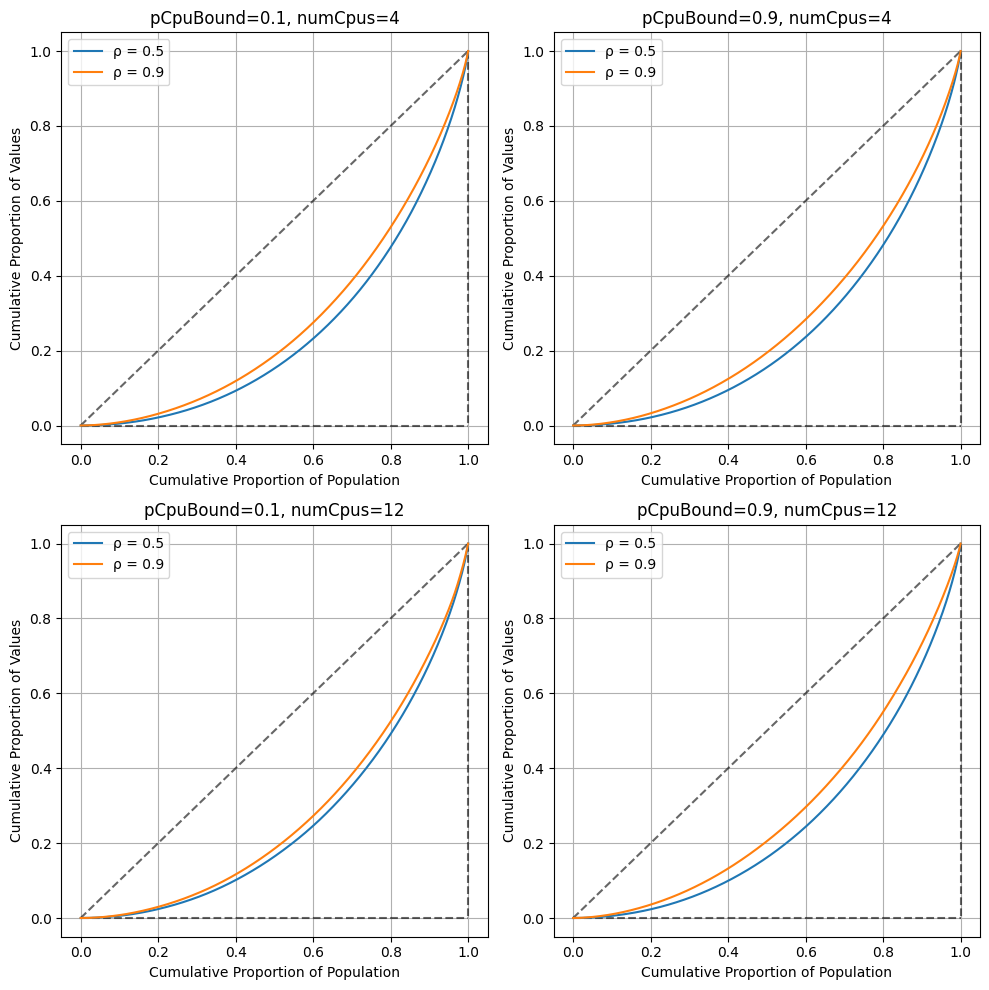
\includegraphics[width=0.7\textwidth]{./images/04/fcfs/turn/lorenz.png}
    \caption{Lorenz curve of the turnaround time of the systems.}
    \label{fig:fcfsTurnLorenz}
\end{figure}

\begin{figure}[H]
    \captionsetup{type=figure}
    \centering
    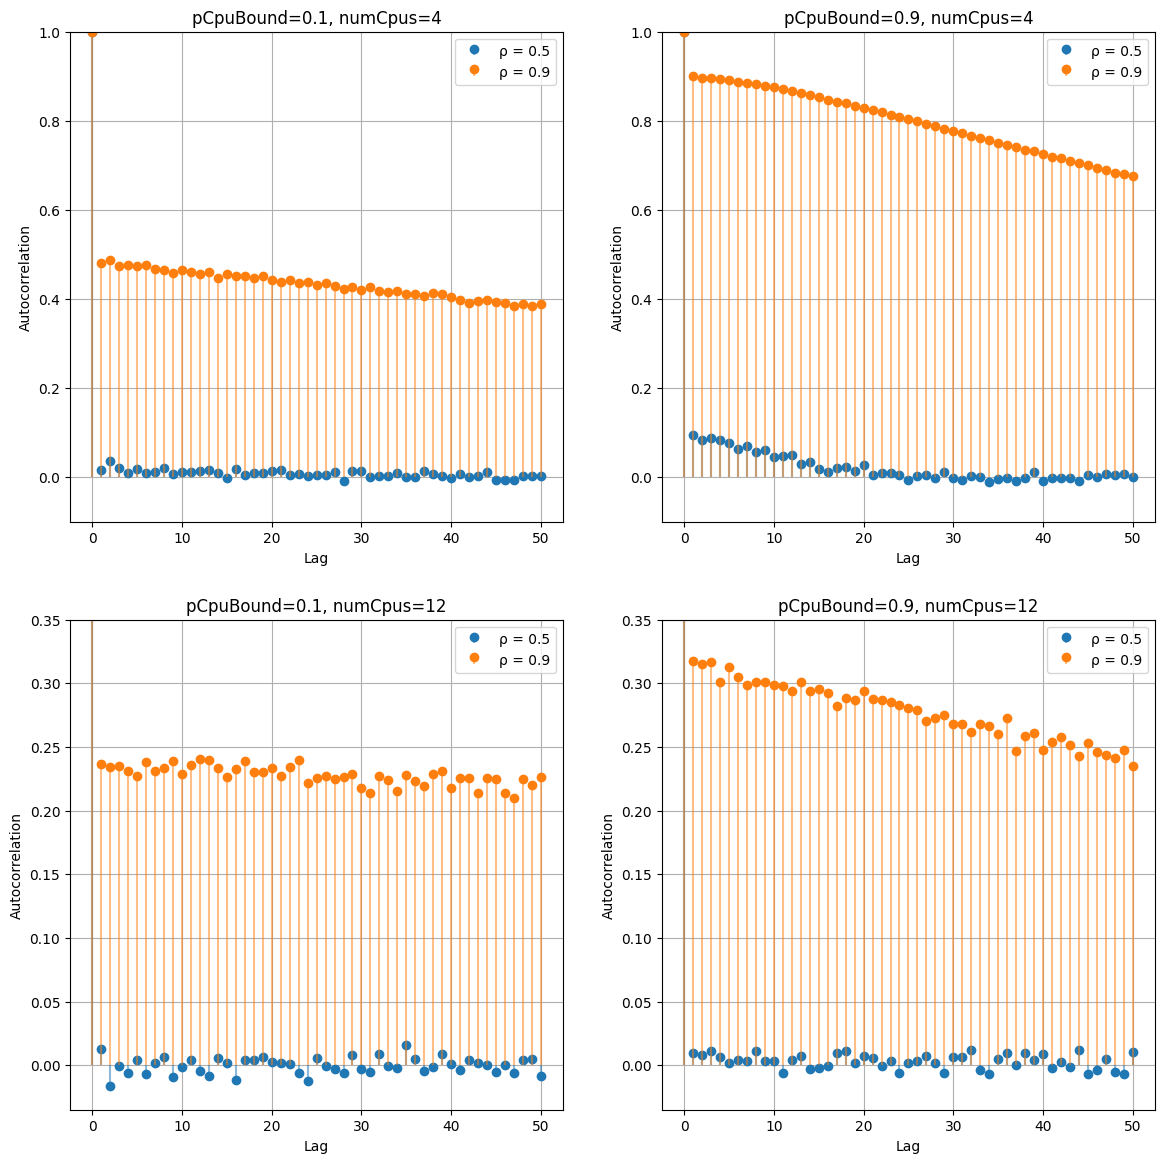
\includegraphics[width=0.7\textwidth]{./images/04/fcfs/turn/autocorrelation.png}
    \caption{Autocorrelation plot of the turnaround time of the systems.}
    \label{fig:fcfsTurnAutocorrelation}
\end{figure}

\newpage
After using subsampling to make the data uncorrelated, we used bootstrap to calculate the confidence intervals of the mean and the standard deviation of the turnaround time. The \texttt{std dev} was calculated since we excpect it to be equal to the mean when the distribution is exponential. It can be seen in \cref{tab:fcfsTurn} that for small $\rho$ they are similar.

\begin{table}[H]
    \centering
    \scriptsize
    \begin{tabular}{llc|c|c|c|c|c|c|c}
\toprule
& & \multicolumn{4}{c|}{numCpus = 4} & \multicolumn{4}{c}{numCpus = 12} \\
& & \multicolumn{2}{c|}{pCpuBound = 0.1} & \multicolumn{2}{c|}{pCpuBound = 0.9} & \multicolumn{2}{c|}{pCpuBound = 0.1} & \multicolumn{2}{c}{pCpuBound = 0.9} \\
Index & & $\rho = 0.5$ & $\rho = 0.9$ & $\rho = 0.5$ & $\rho = 0.9$ & $\rho = 0.5$ & $\rho = 0.9$ & $\rho = 0.5$ & $\rho = 0.9$ \\
\midrule
\multirow{3}{*}{Mean} & Value & 103.1 & 195.0 & 108.5 & 358.4 & 99.6 & 132.5 & 100.1 & 144.6 \\
& 95\% CI Low & 101.2 & 181.2 & 102.3 & 321.2 & 97.7 & 121.5 & 98.6 & 131.4 \\
& 95\% CI High & 105.3 & 211.5 & 114.5 & 395.7 & 101.6 & 146.0 & 101.4 & 158.2 \\
\midrule
\multirow{3}{*}{Std Dev} & Value & 101.3 & 137.2 & 108.1 & 316.6 & 99.3 & 113.5 & 98.8 & 126.7 \\
& 95\% CI Low & 98.6 & 126.2 & 102.2 & 280.2 & 96.7 & 102.4 & 97.0 & 111.8 \\
& 95\% CI High & 104.1 & 152.1 & 115.1 & 365.0 & 102.0 & 127.6 & 100.6 & 145.3 \\
\bottomrule
\end{tabular}
    \caption{Bootstrap results for turnaround time mean and Std Dev. (ms)}
    \label{tab:fcfsTurn}
\end{table}


\subsubsection{Waiting time}

From \cref{fig:fcfsWaitEcdf} and \cref{fig:fcfsWaitDensity} it is clear to see that for $\rho = 0.5$ the waiting time is almost always $0$. For this reason in \cref{fig:fcfsWaitLorenz} we see that the waiting time is more unfair when $\rho$ is lower, since this is the behaviour of the line of maximum unfairness (all values$ = 0$ except for one). In \cref{fig:fcfsWaitAutocorrelation} we see that even when $\rho = 0.5$ the times are really correlated.

\begin{figure}[H]
    \captionsetup{type=figure}
    \centering
    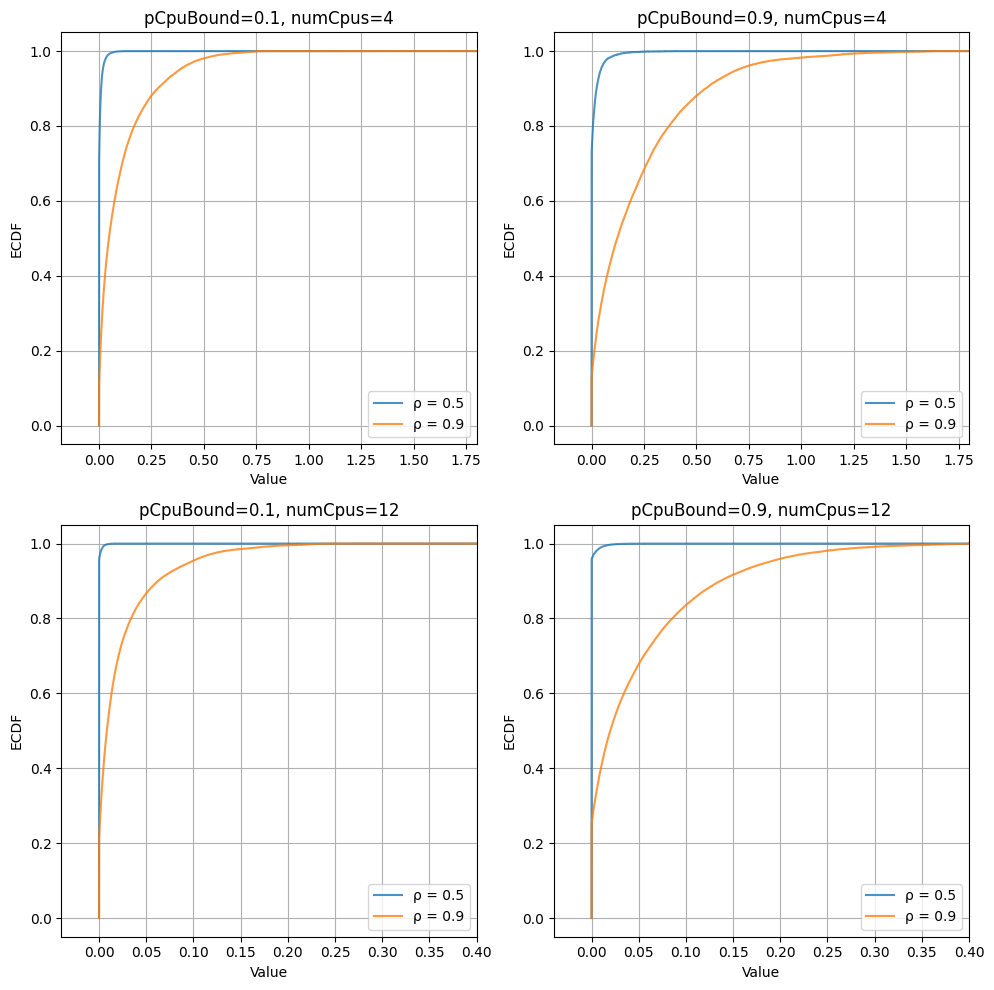
\includegraphics[width=0.85\textwidth]{./images/04/fcfs/wait/ecdf.png}
    \caption{Empirical CDF of the waiting time of the systems.}
    \label{fig:fcfsWaitEcdf}
\end{figure}

\begin{figure}[H]
    \captionsetup{type=figure}
    \centering
    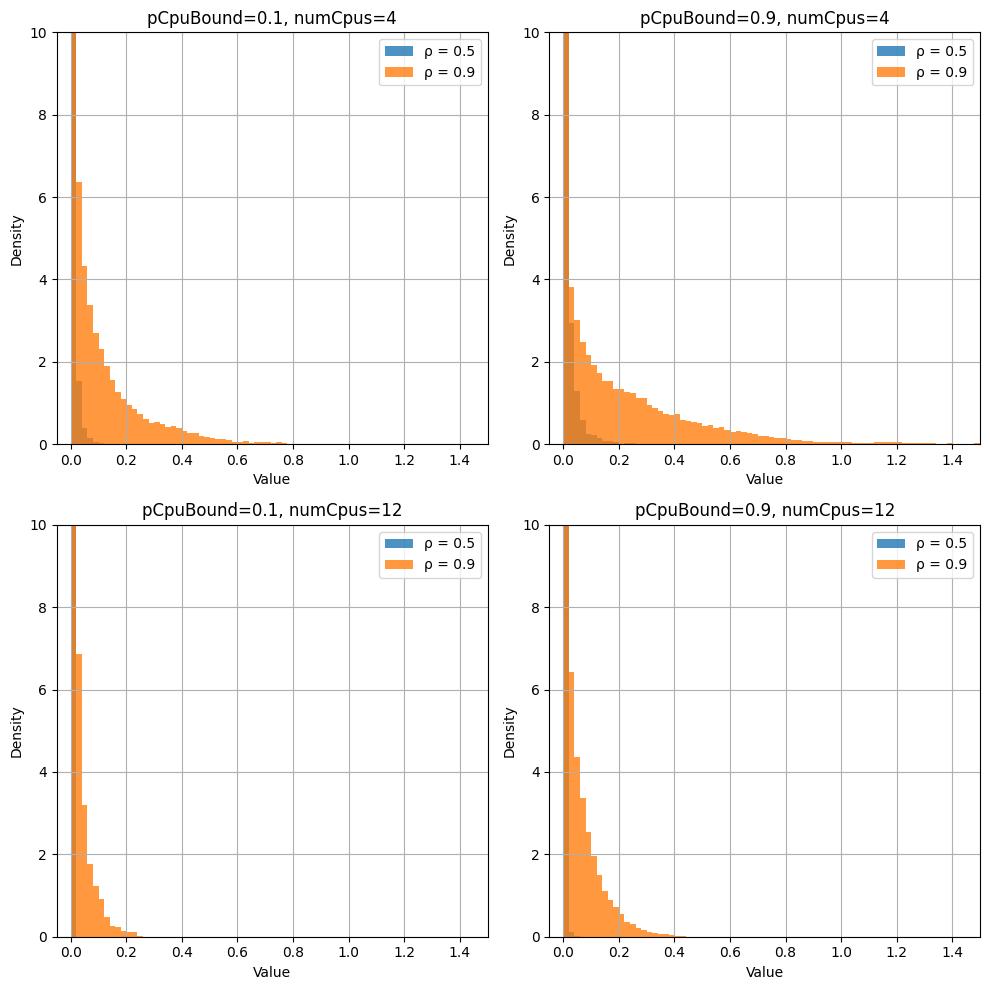
\includegraphics[width=0.7\textwidth]{./images/04/fcfs/wait/density.png}
    \caption{Density plot of the waiting time of the systems.}
    \label{fig:fcfsWaitDensity}
\end{figure}

\begin{figure}[H]
    \captionsetup{type=figure}
    \centering
    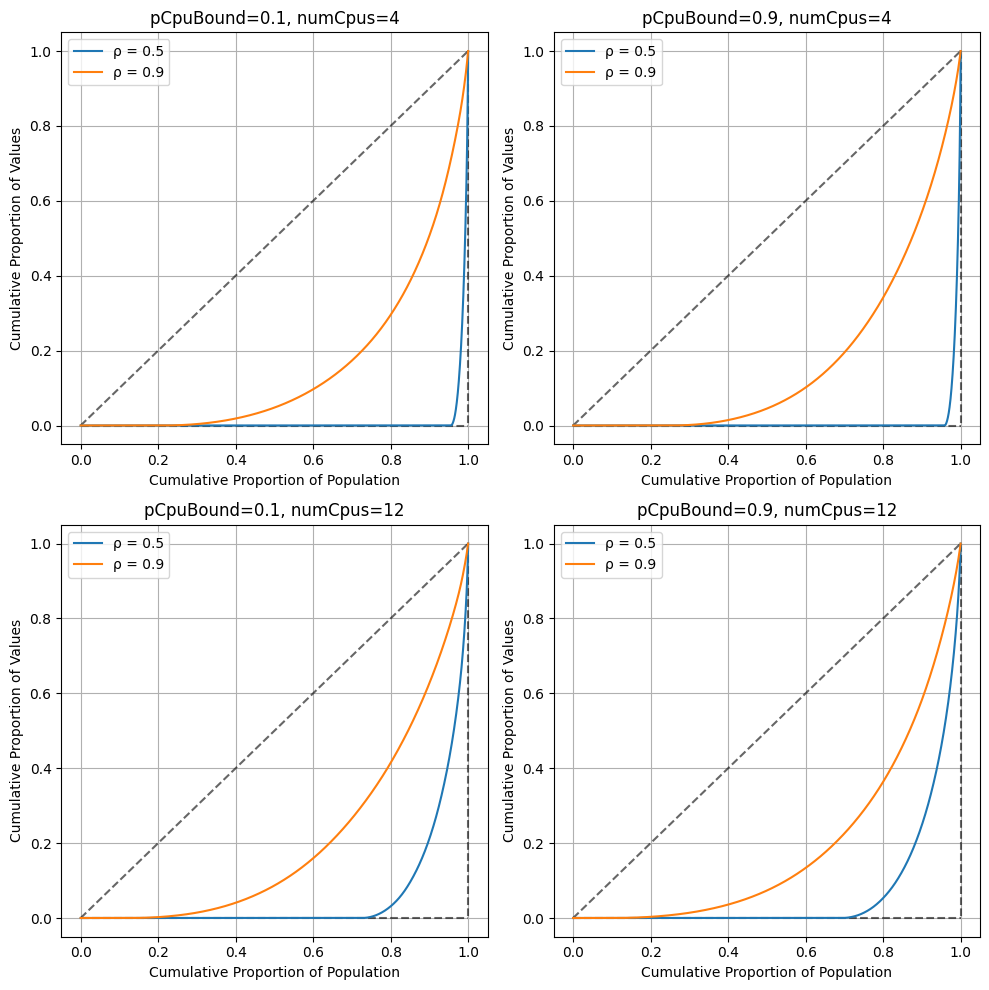
\includegraphics[width=0.9\textwidth]{./images/04/fcfs/wait/lorenz.png}
    \caption{Lorenz curve of the waiting time of the systems.}
    \label{fig:fcfsWaitLorenz}
\end{figure}


\begin{figure}[H]
    \captionsetup{type=figure}
    \centering
    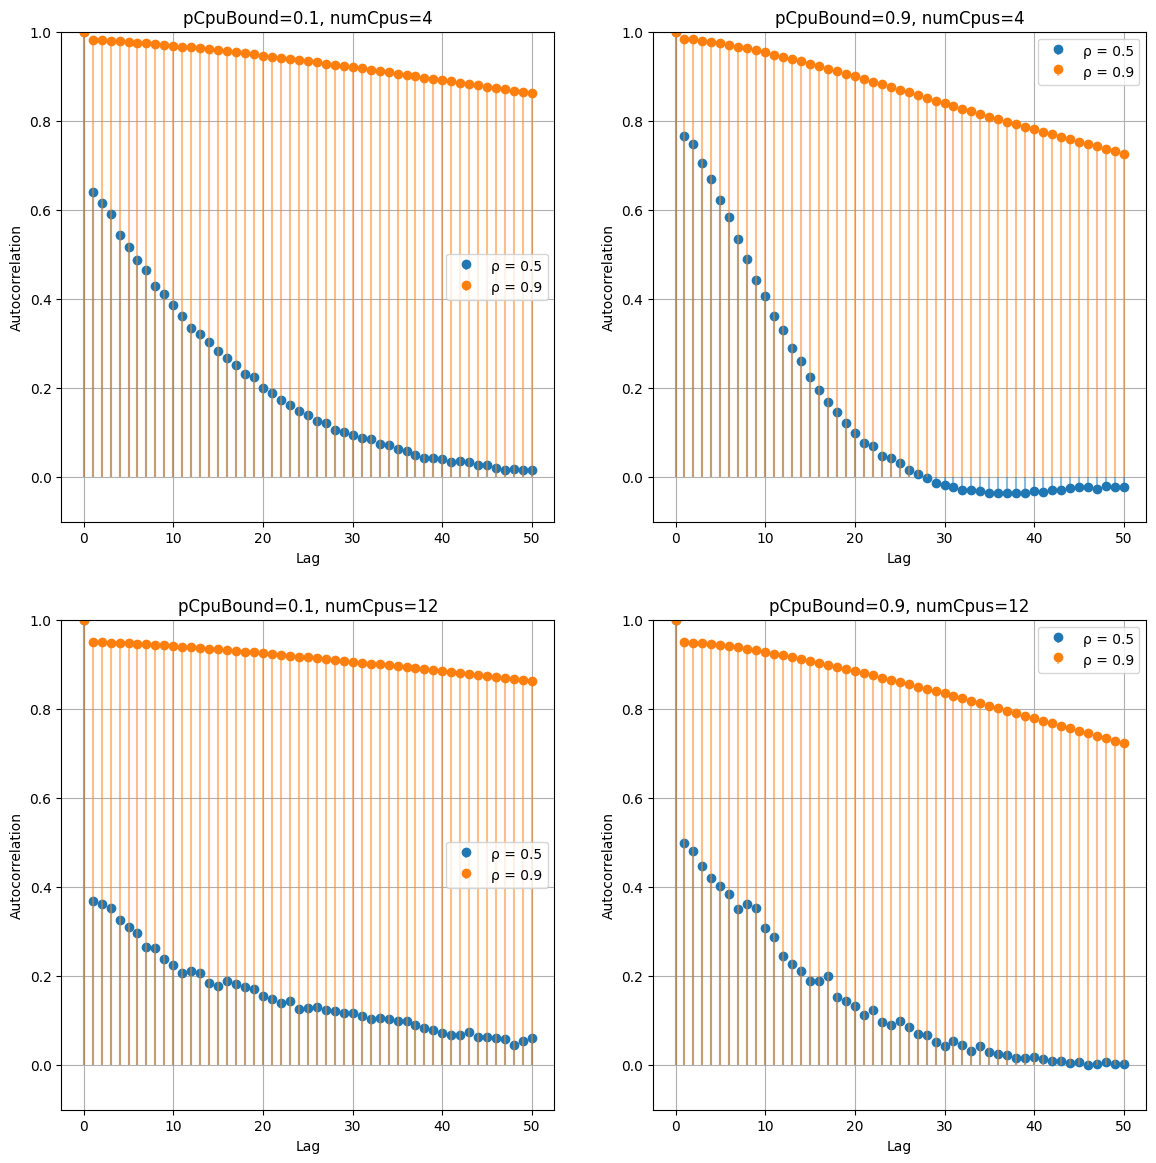
\includegraphics[width=0.7\textwidth]{./images/04/fcfs/wait/autocorrelation.png}
    \caption{Autocorrelation plot of the waiting time of the systems.}
    \label{fig:fcfsWaitAutocorrelation}
\end{figure}



\begin{table}[H]
    \centering
    \scriptsize
    \begin{tabular}{llc|c|c|c|c|c|c|c}
\toprule
& & \multicolumn{4}{c|}{numCpus = 4} & \multicolumn{4}{c}{numCpus = 12} \\
& & \multicolumn{2}{c|}{pCpuBound = 0.1} & \multicolumn{2}{c|}{pCpuBound = 0.9} & \multicolumn{2}{c|}{pCpuBound = 0.1} & \multicolumn{2}{c}{pCpuBound = 0.9} \\
Index & & $\rho = 0.5$ & $\rho = 0.9$ & $\rho = 0.5$ & $\rho = 0.9$ & $\rho = 0.5$ & $\rho = 0.9$ & $\rho = 0.5$ & $\rho = 0.9$ \\
\midrule
\multirow{3}{*}{Mean} & Value & 2.7 & 92.4 & 5.8 & 213.0 & 0.1 & 21.2 & 0.3 & 43.0 \\
 & 95\% CI Low & 2.3 & 81.6 & 4.7 & 186.1 & 0.1 & 18.0 & 0.2 & 36.9 \\
 & 95\% CI High & 3.3 & 103.7 & 8.1 & 242.7 & 0.2 & 25.0 & 0.6 & 50.4 \\
\midrule
\multirow{3}{*}{Std Dev} & Value & 7.8 & 108.9 & 21.5 & 252.7 & 0.9 & 35.4 & 2.2 & 64.8 \\
 & 95\% CI Low & 6.4 & 99.4 & 14.4 & 221.6 & 0.6 & 30.8 & 1.3 & 56.6 \\
 & 95\% CI High & 9.4 & 120.4 & 36.2 & 300.0 & 1.3 & 43.0 & 4.2 & 75.3 \\
\bottomrule
\end{tabular}

    \caption{Bootstrap results for waiting time mean and Std Dev. (ms)}
    \label{tab:fcfsWait}
\end{table}


\subsubsection{CPU utilization}

\label{sec:fcfsCpuUtilization}

\begin{table}[H]
    \centering
    \scriptsize
    \begin{tabular}{lc|c|c|c|c|c|c|c}
\toprule
& \multicolumn{4}{c|}{numCpus = 4} & \multicolumn{4}{c}{numCpus = 12} \\
& \multicolumn{2}{c|}{pCpuBound = 0.1} & \multicolumn{2}{c|}{pCpuBound = 0.9} & \multicolumn{2}{c|}{pCpuBound = 0.1} & \multicolumn{2}{c}{pCpuBound = 0.9} \\
Index & $\rho = 0.5$ & $\rho = 0.9$ & $\rho = 0.5$ & $\rho = 0.9$ & $\rho = 0.5$ & $\rho = 0.9$ & $\rho = 0.5$ & $\rho = 0.9$ \\
\midrule
Mean & 2.02 & 3.61 & 2.03 & 3.63 & 6.01 & 10.82 & 6.03 & 10.80 \\
\midrule
Std Dev & 1.30 & 0.88 & 1.30 & 0.86 & 2.43 & 1.99 & 2.45 & 2.00 \\
\bottomrule
\end{tabular}
    \caption{Mean and Std Dev of number of busy cpus.}
    \label{tab:fcfsCpus}
\end{table}

We see that the obtained values are inline with the theoretical model:
\begin{equation}
    \rho * numCpus = meanCpuUtilized
\end{equation}


For example $0.9 * 4 \approx 3.61$ 

\subsubsection{Ready queue length}

\begin{table}[H]
    \centering
    \scriptsize
    \begin{tabular}{lc|c|c|c|c|c|c|c}
\toprule
& \multicolumn{4}{c|}{numCpus = 4} & \multicolumn{4}{c}{numCpus = 12} \\
& \multicolumn{2}{c|}{pCpuBound = 0.1} & \multicolumn{2}{c|}{pCpuBound = 0.9} & \multicolumn{2}{c|}{pCpuBound = 0.1} & \multicolumn{2}{c}{pCpuBound = 0.9} \\
Index & $\rho = 0.5$ & $\rho = 0.9$ & $\rho = 0.5$ & $\rho = 0.9$ & $\rho = 0.5$ & $\rho = 0.9$ & $\rho = 0.5$ & $\rho = 0.9$ \\
\midrule
Mean & 0.25 & 13.72 & 0.22 & 10.27 & 0.03 & 9.81 & 0.03 & 7.19 \\
\midrule
Std Dev & 0.96 & 18.47 & 0.89 & 12.99 & 0.29 & 16.34 & 0.28 & 10.57 \\
\bottomrule
\end{tabular}

    \caption{Mean and Std Dev of number of ready processes in queue.}
    \label{tab:fcfsReadyProc}
\end{table}
